\documentclass[12pt,letterpaper]{article}
%\usepackage[margin=1.5in]{geometry} % Set page margin
\usepackage{etex}
\usepackage[T1]{fontenc}
\usepackage{amsmath}
\usepackage{amsfonts}
\usepackage{amssymb}
\usepackage{graphicx}
\usepackage{url}
\usepackage{nth}
\usepackage{fixltx2e}
\usepackage{listings}
\usepackage{appendix}
\usepackage{courier}
\usepackage{multicol}
\usepackage{multirow}
\usepackage{adjustbox}
\usepackage[table]{xcolor}% http://ctan.org/pkg/xcolor
\usepackage[htt]{hyphenat}
\usepackage[bottom]{footmisc} % Keep footnotes stuck to the bottom
\usepackage{epigraph}
\usepackage{marginnote}
\usepackage{float}
\usepackage{pgfplots}
\usepackage{pgfplotstable}
\usepackage{tikz}
\usetikzlibrary{shapes,arrows}
\usepackage{draftwatermark}
\usepackage{tabularx,ragged2e,booktabs,caption}
\usepackage{xspace}
\newcolumntype{C}[1]{>{\Centering}m{#1}}
\renewcommand\tabularxcolumn[1]{C{#1}}
\SetWatermarkColor[rgb]{1,0.85,0.85}
\interfootnotelinepenalty=10000 % Don't split footnotes accross pages.
%-------------------------------------------------
% From http://tex.stackexchange.com/a/60212/31317
\usepackage{titlesec}
\usepackage[pdfpagelayout=TwoPageRight]{hyperref}
\usepackage{fontspec}

\setmainfont[Ligatures=TeX]{Times New Roman}
\setmonofont[Scale=MatchLowercase]{DejaVu Sans Mono}

% Signature and date command.
%\newcommand*{\SignatureAndDate}[1]{%
%    \par\noindent\makebox[2.5in]{\hrulefill} \hfill\makebox[2.0in]{\hrulefill}%
%    \par\noindent\makebox[2.5in][l]{#1}      \hfill\makebox[2.0in][l]{Date}%
%}%

\titleclass{\subsubsubsection}{straight}[\subsection]

\newcounter{subsubsubsection}
\renewcommand\thesubsubsubsection{\thesubsubsection.\arabic{subsubsubsection}}
\renewcommand\theparagraph{\thesubsubsubsection.\arabic{paragraph}} % optional; useful if paragraphs are to be numbered

\titleformat{\subsubsubsection}
  {\normalfont\normalsize\bfseries}{\thesubsubsubsection}{1em}{}
\titlespacing*{\subsubsubsection}
{0pt}{3.25ex plus 1ex minus .2ex}{1.5ex plus .2ex}

\makeatletter
\renewcommand\paragraph{\@startsection{paragraph}{5}{\z@}%
  {3.25ex \@plus1ex \@minus.2ex}%
  {-1em}%
  {\normalfont\normalsize\bfseries}}
\renewcommand\subparagraph{\@startsection{subparagraph}{6}{\parindent}%
  {3.25ex \@plus1ex \@minus .2ex}%
  {-1em}%
  {\normalfont\normalsize\bfseries}}
\def\toclevel@subsubsubsection{4}
\def\toclevel@paragraph{5}
\def\toclevel@paragraph{6}
\def\l@subsubsubsection{\@dottedtocline{4}{7em}{4em}}
\def\l@paragraph{\@dottedtocline{5}{10em}{5em}}
\def\l@subparagraph{\@dottedtocline{6}{14em}{6em}}
\makeatother

\setcounter{secnumdepth}{4}
\setcounter{tocdepth}{4}
%-------------------------------------------------
\author{Michael Holler}
\title{Automated Textbook Indexing with Na\"ive Bayes Classifier Trained on Wikipedia Articles}
\begin{document}
\pagenumbering{gobble}
\makeatletter
\begin{titlepage}
\begin{center}
{\LARGE \@title}

\vspace{1in}
{\Large \@author}

\vspace{1in}
\textsc{\LARGE Senior Honors Thesis}

\vspace{0.3in}
Submitted in Partial Fulfillment of Requirements of the\\
{\it College Scholars Honors Program}\\
{\it North Central College}

\vspace{1in}
\@date

\vspace{1in}
\begin{tabular}{llll}
Approved: & $\underset{\text{Thesis Director Signature}}{\line(1,0){150}}$ & Date: & \line(1,0){70} \\[1.45ex] 
& \multicolumn{1}{c}{{\footnotesize Dr. Caroline St. Clair}} && \\ 
\end{tabular}

\vspace{0.35in}
\begin{tabular}{llll}
Approved: & $\underset{\text{Thesis Director Signature}}{\line(1,0){150}}$ & Date: & \line(1,0){70} \\[1.45ex] 
& \multicolumn{1}{c}{{\footnotesize Dr. Michael De Brauw}} && \\ 
\end{tabular} 

%Approved: $\underset{\text{Thesis Director Signature}}{\line(1,0){150}}$ \quad Date: %\line(1,0){70}

%\vspace{0.25in}
%Approved: $\underset{\text{Second Reader Signature}}{\line(1,0){150}}$ \quad Date: \line(1,0){70}

%{\LARGE Senior Honors Thesis}
\end{center}
\end{titlepage}
\makeatother

\clearpage\mbox{}\clearpage

\epigraph{You want weapons? We're in a library! Books! The best weapons in the world! This room's the greatest arsenal we could have---arm yourselves!}{---The Doctor}
\epigraph{Automatic indexing of books has failed miserably, as will be discussed below.}{---Nancy Mulvany, {\it Indexing Books}}
\epigraph{The idea behind digital computers may be explained by saying that these machines are intended to carry out any operations which could be done by a human computer.}{---Alan Turing}
\pagebreak
\pagenumbering{roman}
\tableofcontents

\clearpage\mbox{}\clearpage % Get TOC to show up on right facing page.

\phantomsection
\addcontentsline{toc}{section}{Acknowledgements}
\begin{center}
\textbf{\Large Acknowledgements}
\end{center}

Placeholder. This will be a surprise :)
%I would like to express my deep gratitude to Dr. Caroline St. Clair, my thesis director, for her constant encouragement and invaluable feedback throughout this research.
%I would also like to thank Dr. Michael De Brauw for his feedback as my second reader, and John Small for his help verifying my references.

%Finally, I would like to thank my parents and girlfriend for their extensive support, encouragement, and understanding over the past year.

\newpage
\thispagestyle{empty}
\mbox{}

\cleardoublepage
\pagenumbering{arabic}
\lstset{
	basicstyle=\ttfamily,
	showstringspaces=false,
	numberstyle=\tiny,
	numbersep=10pt,
	numbers=left,
	stepnumber=1,
	frame=single,
	aboveskip=0.5cm,
	belowskip=0.5cm
}
\newpage
\begin{abstract}
Lorem ipsum dolor sit amet, consectetur adipiscing elit. Praesent auctor augue eu ipsum vulputate malesuada. Quisque scelerisque, ante id egestas congue, nibh erat adipiscing odio, sit amet iaculis velit ante non metus. Phasellus enim dolor, auctor eu tempus vitae, hendrerit vitae nisi. Proin commodo magna a metus consequat interdum. Sed pharetra eget felis nec mollis. Mauris cursus dolor faucibus elementum imperdiet. Aenean in fringilla nulla. Donec vulputate risus sed sapien venenatis dignissim. Vestibulum ac tortor non purus viverra tristique. Morbi sed bibendum metus.
\end{abstract}
% Where to put why I decided to use paragraphs for context instead of pages?
\section{Introduction}

The number of books published in the U.S. has been on the rise for at least the past decade, only incurring a small setback in 2005\cite{bowker}.
In 2010, Bowker recorded 328,259 new books published in the United States---up from 302,410 during the previous year.
Despite concerns that the paper book is on it's way out, the book publishing industry is still very much a growing one.

% New Books Published per Year Graph
\begin{center}
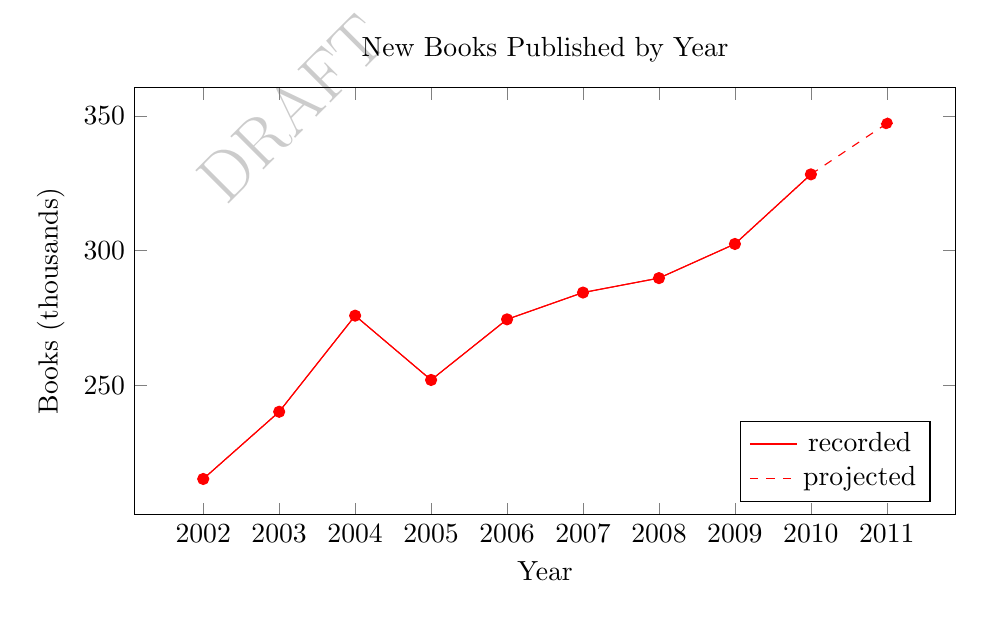
\begin{tikzpicture}
	\begin{axis}[
		title={New Books Published by Year},
		xlabel={Year},
		xticklabel style={/pgf/number format/1000 sep=},
		ylabel={Books (thousands)},
		width=12cm,
		height=7cm,
		legend pos=south east]
		
		\addplot[color=red,mark=,line join=round, solid] coordinates {
			(2002,215.138)
			(2003,240.098)
			(2004,275.793)
			(2005,251.903)
			(2006,274.416)
			(2007,284.370)
			(2008,289.729)
			(2009,302.410)
			(2010,328.259)
		};
		\addplot[color=red,mark=,line join=round, dashed] coordinates {
			(2010,328.259)
			(2011,347.178)
		};
		\addplot[color=red,mark=*,line join=round, solid] coordinates {
			(2002,215.138)
			(2003,240.098)
			(2004,275.793)
			(2005,251.903)
			(2006,274.416)
			(2007,284.370)
			(2008,289.729)
			(2009,302.410)
			(2010,328.259)
		};
		\addplot[color=red,mark=*,line join=round, dashed] coordinates {
			(2011,347.178)
		};
		
		\addlegendentry{recorded}
		\addlegendentry{projected}
	\end{axis}
\end{tikzpicture}
\end{center}

It's a fair assumption that many of these new books also contain an index section between their covers.
An index, of course, is, ``An alphabetical list, placed (usually) at the end of a book, of the names, subjects, etc. occurring in it, with indication of the places in which they occur,'' \cite{oed-index}.
Indexes are popular in non-fiction books, particularly in textbooks.
Readers use indexes to quickly and efficiently locate passages of the book focusing on a specific topic.
Thus, it is important for a book's index to be of high quality, so the reader can locate a particular topic with ease.
A good index can make learning and research easy, while a bad index can result in readers' frustration as they scan over each page in an attempt to find what they are looking for.

\subsection{Cost of Indexing}

The growing number of books published each year and the need for quality indexes in books of all types makes indexing an important sub-industry of the publication process.
Since many books contain indexes, any change in the indexing industry directly affects the publication industry.
If indexing could be made more efficient, the publishing industry could allocate the significant resources that would have gone toward indexing to other, more productive areas.

In {\it Indexing Books}, Nancy Mulvany writes that, ``a typical three-hundred-page book can easily cost close to a thousand dollars to index.
This was in 1994.
Adjusted for inflation using the U.S. Bureau of Labor Statistics' online calculator, \$1,000 dollars in 1994 is equivalent to \$1,578.38 in 2014\cite{inflation-calculator}.
Mulvany goes on to estimate the typical price-per-page at three 1993 U.S. dollars per page in 1994\cite{mulvany}, which is equivalent to \$4.74 in 2014\cite{inflation-calculator}.

The amount of time and money spent on indexing annually can be quantified if a few simplifying assumptions are established.
All rows without citations are conservative guesses for the purpose of estimation:

\begin{center}
\begin{tabular}{|c|l|l|}
\hline
\multicolumn{1}{|c|}{{\bf Symbol}} & \multicolumn{1}{c|}{{\bf Description}} & \multicolumn{1}{c|}{{\bf Statistic}} \\
\hline
$b$ & Number of books published in 2010 \cite{bowker} & 328,259 books \\
\hline
$c$ & Percentage of Books requiring Indexes & 15\% \\
\hline
$d$ & Average dollars per page indexed \cite{mulvany,inflation-calculator} & \$4.74 \\
\hline 
$p$ & Average Number of Pages in Book & 300 pgs \\ 
\hline 
$r$ & Average Number of Pages Indexed per Hour \cite{connolly} & 7 pgs/hr \\
\hline
\end{tabular}
\end{center}

Given these variables, equations are developed to calculate average cost and time impact of manual indexing.

\begin{figure}[H]
$$ \text{cost} = b \times c \times p \times d $$
$$ \text{time} = \frac{b \times c \times p}{r} $$
\\
$$ 69,377,744.70 \text{ USD} = 328259 \times 0.15 \times 300 \times 4.74 $$
$$ 240 \text{ years}= 2,110,236.48 \text{ hours} = \frac{328259 \times 0.15 \times 300}{7}$$
\caption{The Price of Manual Indexing}
\end{figure}

Even with the very conservative assumptions that the average book contains 300 pages and 15\% of books require indexes, the cost of indexing new US books in 2010 was incredibly high.
These numbers reveal the economic impact of indexing, but the individual impact is important too.
If an author wants to index his or her own book, it would take about 42 hours on average. The author could devote an entire work week towards something more productive if there existed an easier way to generate an index.
Clearly, indexing is a significant part of the publishing industry.
natural language processing, a growing specialization of computer science, might be able to reduce these high costs.

\begin{figure}
$$ 42 \text{ hours} = \frac{300}{7} = \frac{p}{r}$$
\end{figure}

\subsection{Natural Language Processing}
% Talk about the rise of natural language processing.

Natural language processing (NLP) is, ``a form of computational linguistics in which natural-language texts are processed by computer (for automatic machine translation, literary text analysis, etc.)''\cite{oed-nlp}.
The sub-discipline of natural language processing (NLP) has existed since the beginning of computers themselves (around 1940), but it has not existed in the modern sense until more recently.
Today, there is a growing focus on machine learning algorithms and processing large amounts of textual data\cite{jurafsky}.
Internet search engines like Google rely on NLP techniques to generate their search results\footnote{As of March 1, 2014, Google has published 219 whitepapers on NLP topics, principally how to use NLP to improve search results.\cite{google-nlp}}, text editing software uses NLP to detect grammatical errors in sentences\cite{norvig}, and mobile applications use NLP to extract summaries from long form text\cite{bit-of-news}.




\section{Background}
% Background section placeholder (move everything below this to another file eventually).
The process of creating an index is either costly or time consuming for authors, depending on whether they choose to create the index themselves or pay someone to do it.
The act of creating an index is labor and organization intensive, often requiring a text to be read multiple times while keeping track of entries electronically or on index cards.

Since indexing a book is so expensive and time consuming, it makes sense to see if computers can be used to generate an index that is nearly as accurate as human indexing professionals.
To automate the indexing process, software exists to replace the indexer's index cards with a more efficient computerized organization system.
However, there is a new, rising interest in seeing if computers can generate indexes deterministically, without the help of human beings.
To do this, software engineers and researchers must apply natural language processing techniques in new and interesting ways.
Before any application, one must understand how well humans can generate indexes to understand how accurate computer need to be in order to match them.

\subsection{Accuracy of Human and Automatic Indexes}

In {\it Natural-Language Processing and Automatic Indexing}, an article published in {\it The Indexer} by C. Korycinski and Alan F. Newell, the authors cite relevant metrics for automatic indexing excerpted from Cleverdon's work:

\begin{quote}
\begin{enumerate}
\item if two people or groups of people construct thesauri in a given subject area, only 60\% of the index terms may be common to both;
\item if two experienced indexers index a given document using a given thesaurus, only 30\% of the index terms may be common to the two sets;
\item if two intermediaries [person who undertakes a database search on behalf of the user] search the same question on the same database on the same host, only 40\% of theoutput may be common to both searches;
\item if two scientists or engineers are asked to judge the relevance of a given set of documents to a given question, the area of agreement may not exceed 60\%.\cite{automatic-indexing}
\end{enumerate}
\end{quote}

Of course, 2 is most relevant, but the other three reveal how imprecisely human beings perform tasks that replicate another human's work.
In the statistics given above, indexing is the least precise of all of the human classification tasks mentioned above.
This makes the number to match for an automatic indexer 30\%.
That is, a computer index compared to a human index should display the same proportion of similarity as a human generated index compared to another human generated index.
Now that a metric for index quality has been established, the next section backgrounds methods and strategies that can be used to create an automatic indexer that might be able to match this benchmark.

\subsection{Natural Language Processing}

Natural language processing (NLP) is, ``a form of computational linguistics in which natural-language texts are processed by computer (for automatic machine translation, literary text analysis, etc.)''\cite{oed-nlp}.
Essentially, it is the area of study in computer science where language and logic meet.
The sub-discipline of natural language processing (NLP) has existed since the beginning of electronic computers themselves (around 1940), but it has not existed in the modern sense until more recently.
Today, there is a growing focus on teaching computers to understand and learn the desired qualities of a text so they can be analyzed and extracted from large amounts of textual data\cite{jurafsky}.

Internet search engines like Google rely on NLP techniques to generate their search results\footnote{As of March 1, 2014, Google has published 219 whitepapers on NLP topics, primarily on how to use NLP to improve search results.\cite{google-nlp}}, text editing software uses NLP to detect grammatical errors in sentences\cite{norvig}, and mobile applications use NLP to extract summaries from long form text\cite{bit-of-news}.

\subsubsection{Machine Learning}

The process of teaching computer to learn and understand information is called machine learning.
Computer learning sounds complicated, but ultimately machine learning is about programming computers to answer questions about new, previously unseen data by correlating it to data it has previously seen, or {\it trained} on.
In {\it Natural Language Processing with Python}, an introductory NLP textbook, the authors use the example of name genders ({\it e.g.}, {\it Mike} is male and {\it Valerie} is female) to help readers understand how machine learning is used to help computers understand language\cite{nlpwp}.
Given a list of names, a computer can be taught to determine (with reasonably high accuracy) whether a new, unseen name is masculine or feminine.
English readers use certain heuristics (shortcuts) to aid in determining the gender of a name, and computers can do the same.
For example, an average person might know that names ending in {\it -a} are typically feminine, while names ending in {\it -o} are typically masculine, so he or she understands that the last letter is a strong determinant of a name's gender, or {\it label}.
In NLP, these determinants are known as {\it features}.
With enough data about names and their genders (a {\it training set}), the probability of a letter determining a particular gender can be calculated, and a person could be {\it trained} using this data and the "last letter" feature to guess name genders with reasonable accuracy.
Of course, the last letter is not the only feature of a name that determines its gender, and by training with additional relevant features the classifier's guesses can be made more accurate.
Indeed, this process of determining the category (or {\it class}) of an item is called {\it classification}.
The above is an example a {\it supervised} machine learning, since training data is involved.
Unsupervised machine learning algorithms are outside the scope of this research, and will not be mentioned further in this paper.

\subsubsection{Document Classification}
% Document classification and automatic indexing
Document classification is a type of NLP that uses machine learning methods like those above, and is used in this research to create a computer generated index.
Document classification involves taking a piece of text (known as a {\it document}) as input and producing a label or {\it class} as output\cite{jurafsky}%.
Determining a name's gender can be thought of as document classification on a very small scale; a ``document'' in that case is a single name.
When applying document classification to automatic indexing, the size of the input documents must be defined.
Since classifiers label every input document with the most probable class\footnote{Classifiers do not have an ``unsure'' or ``ambiguous'' category; if the gender of a particular name is confusing, it is still assigned a gender according to the gender that is most likely, even if it is only slightly more likely than another gender.} the size of the document should be the smallest piece of text likely to contain an index reference.
Since no research recommending a document size for automatic indexing tools exists, this research elects to use paragraphs as documents, such that a book containing $n$ paragraphs would be split up into $n$ unique documents.

Selecting a document size creates room for error, since one paragraph ought not to have any index references, and another might have more than one.
This is a problem, because a document classifier assigns each document one and only one class.
While typically a paragraph will likely only have one index reference, the uncommon but possible cases of $r = 0$ and $r > 1$, where $r$ represents the number of references in a paragraph, must be handled gracefully and consistently.
The parameters for success in each of these cases are defined below:

\begin{itemize}
\item In the trivial $r = 1$ case, a document is successfully labeled when it is labeled with the same class as the human generated index for the same text.
\item In the case of $r > 1$, this research considers a document successfully labeled if it is assigned one of the same index labels as the source text's index.
\item In the case of $r = 0$, a document can never be successfully labeled, since the classifier must assign the document a class and ``none'' is not an option. This limitation is disappointing, but impossible to avoid when using document classifiers.
\end{itemize}

This research makes the overarching that a book with $n$ paragraphs has $n$ index references, or page number references in the book's index.
Clearly, this is an unrealistic assumption, but when dealing with document classification it is an assumption that must be made.

To clarify terminology, this index is considered to have two index entries or labels, and five index or page number references:

\begin{center}
\textit{aardvark} 12, 32, 54, 67 \\
\textit{apple}, 34
\end{center}

\noindent This does {\it not} mean that a book is assumed to have $n$ unique words or phrases in its index, just that the collection of index words and phrases {\it points to} $n$ pages, since a singular index word might be referenced in multiple places (as seen in {\it aardvark} above).

\subsubsection{Na{\"i}ve Bayes Classifiers}

There are many different methods of classification, including decision trees, na{\"i}ve Bayes, and maximum entropy classifiers\cite{nlpwp}, but this research only evaluates efficacy of the na{\"i}ve Bayes classifier in the task of automated indexing.
As far as classifiers go, \naive Bayes is one of the simplest implementations\cite{rish}.
How it functions is described below:
\begin{quote}
The \naive Bayes classifier begins by calculating the prior probability of each label, which is determined by checking the frequency of each label in the training set. The contribution from each feature is then combined with this prior probability, to arrive at a likelihood estimate for each label. The label whose likelihood estimate is the highest is then associated to the input value.\cite{nlpwp}
\end{quote}
\noindent Once trained, each feature is assigned one label.
In classification, any occurrence of a feature will ``push'' the document further towards the feature's assigned label.
When a feature ``pushes'' a document towards another label, it also pushes it towards similar labels, and an equal-but-opposite reaction hurts labels that are dissimilar from the occurring feature's label.

The decision to use \naive Bayes primarily motivated by simplicity, but it is important to acknowledge that this simplicity comes with a small cost in accuracy.
Since little research has been done on the use of document classification for automatic index generation, it made sense to begin with a simple implementation of such a classifier before even considering to work with something more complex like the maximum entropy classifier.
\Naive Bayes is considered simple because it makes a strong assumption that all features are independent from one another, that the appearance of one feature does not affect the possibility that another will appear.
This assumption is unrealistic as the probability of one feature might increase or decrease if another feature is present, creating an instance of conditional probability.
Ignoring conditional probability can lead to a phenomena called double counting.
This phenomena can be clearly seen if two features ``contains(apple)'' and ``contains(gala apple)'' are present in the same feature set.
The probability of ``apple'' occurring if `gala apple'' has already occurred is 1, and conversely the probability of ``gala apple'' occurring is increased when ``apple'' is present.
Although \naive Bayes' independence assumption does have some bearing on the result of the classification, research shows that this affect is largely negligible for most feature and data sets.

Irene Rish affirms in an IBM white paper that \naive Bayes works well with completely independent features {\it and} functionally dependent features (which should be surprising).
Her research also notes that, ``a better predictor of \naive Bayes accuracy is the amount of information about the class that is lost because of the independence assumption''\cite{rish}.
These findings suggest that \naive Bayes should prove to be a sufficiently accurate predictor of the efficacy of using document classification for automatic indexing, despite the assumptions the algorithm makes about independence.

After deciding upon \naive Bayes, the next step for this research was to select an implementation of the algorithm to use for analysis.

\subsubsection{Natural Language Toolkit}
\label{sec:nltk}

Many different libraries of machine learning and NLP tools\cite{stanford-nlp,open-nlp} exist, this research selected Python's Natural Language Processing Toolkit (NLTK) library\cite{nltk} for its popularity, flexibility, large selection of both NLP and machine learning tools, thorough documentation, and ease of use.

Publicly released in 2009, NLTK has become a staple in the world of NLP.
Even with well over 4,000 Python packages in the Python Package Index (PyPI), PyPI Ranking cites NLTK as having over 180,000 downloads, making it the \nth{273} most downloaded Python package of all time, and Python's most popular NLTK package\cite{pypi-ranking}.
The latest available stable version of NLTK (v2.0.4) was used for the entirety of this research.

Python, the language NLTK is written for, is used for data analysis throughout this research.
Python is a mature and robust high-level scripting and prototyping language, and is therefore well-suited to the task of exploratory research.
This research uses the latest version of Python 2, since NLTK only provides alpha-level support for Python 3\cite{nltk-install}.
\section{Data Collection}

This research leverages supervised learning algorithms, meaning it requires a training set and a test set to develop an appropriate feature set to use in conjunction with the supervised learning algorithm.
The training set allows the algorithm to ``learn'' how to classify different sections of text, and the test set is used to validate that documents are classified correctly.
Unlike most implementations of supervised learning algorithms, the test and training set data come from different sources.
Wikipedia is used for the training set, and a PDF textbook is used for test data.
The following sections contain justification for the choice of data to used for each set, and the methods used to structure and collect that data for analysis.

\subsection{Test Set}

Since the goal of this research is to create an index for a book, the test set is generated from a textbook with a comprehensive index section.
This textbook is called {\it Biology} \cite{biology}, and is freely available from OpenStax \cite{openstax-bio} under the Creative Commons Attribution license.
The book was created by six senior contributors that hold professorial positions at prevalent universities, and approximates an average college textbook.
This textbook is 1477 pages long, containing an index of 3118 unique topics (labels) making for 4678 different index entries (references).

In {\it Biology}, all words referred to by index entries are bolded in the text itself. Below is an example of what this looks like (bold in original):

\begin{quote}
Symbiotic relationships, or symbioses (plural), are close interactions between individuals of different species over an extended period of time which impact the abundance and distribution of the associating populations. \cite{biology}
\end{quote}

\noindent Here, the bold word ``symbioses'' is referred to by an index entry at the back of the book with the same name. All index entries point to bold words, and all bold words point to index entries. This fact makes it trivial to find which part of the page an index reference is referring to, making it a good candidate for test data.

\subsubsection{Structuring the Test Data}

Useful though {\it Biology} is as a data source, it is not available in a structured, easily parsable format.
In order to make the data in {\it Biology} useful, it needs to be converted from it source PDF into a structured form.
To do this, a relational database is used to store the book's text alongside meta data like page number and paragraph location.

\subsubsection{Importing Index Entries into Relational Database}

To expedite the structuring process, text was copied manually from the PDF, and pasted into a plain text document.
Regular expressions were used to massage the data into a simple, comma separated format.
In this format, each line represents a unique index entry, with the first column in a line holding the index label (or name), and each subsequent column holds a page number the label can be found on.
Now that the data are more easily parsable, there must be a way to it in a relational database for analysis purposes.

It is important to create a table to hold the index labels separate from the page numbers, since one label can refer to multiple pages.
In this table, indexId is an autoincrementing ID, label is the name of the index entry as it appears in the book (e.g., ``Acid rain''), and wikiLabel is the label if the label were a wikipedia article name (e.g., ``Acid\_rain'') which is achieved by replacing spaces in the label with underscores.

\begin{center}
\begin{tabular}{|c|}
\hline 
\textbf{index} \\ 
\hline 
bookId \\ 
\hline 
indexId \\ 
\hline 
label \\ 
\hline 
wikiLabel \\ 
\hline 
\end{tabular}
\end{center}
 
An indexedPage table must exist to store index references (page numbers) that belong to index labels.
This table simply contains an indexId and a pageNum, which allows for joins onto the index table to replicate the whole index.

\begin{center}
\begin{tabular}{|c|}
\hline 
\textbf{indexedPage} \\ 
\hline 
indexId \\ 
\hline 
pageNum \\ 
\hline 
\end{tabular} 
\end{center}

Once these tables are created, the structured CSV file can be imported using the custom indexImporter.php (see Appendix B) tool written specifically for this purpose.

The importer script populates all of the columns in both tables with all of the data in the CSV file.

\subsubsection{Reducing Index Entry Set}
\label{subsec:reducing}

Only index entries whose {\tt wikiLabel} value matches a Wikipedia page will be used in the analysis portion of this research.
This means that information need only be gathered from index entries that match this criteria.
To discover this subset of index entries, a database of Wikipedia titles must be intersected with the {\tt index}.

The Wikimedia Foundation periodically creates dumps for their many databases and makes them publically available online\cite{wiki-dumps}.
One of the many data sets they make available is a list of Wikipedia article titles in the main \url{/wiki/} namespace for the English language version of Wikipedia\cite{wiki-dump-titles}.
At the time of this writing, there are 10639771 separate Wikipedia article titles matching this criteria.
This dump will serve as the source that will ultimately be intersected with the {\it Biology} index entries to yield the entries that will be used in analyses.

Before performing this intersection, the English Wikipedia title information must be extracted from the dump file and placed in a table in the relational database.
This table contains a unique {\tt titleId} integer key and a textual {\tt title} in each row.

\begin{center}
\begin{tabular}{|c|}
\hline 
{\bf articleTitles} \\ 
\hline 
titleId \\ 
\hline 
title \\ 
\hline 
\end{tabular} 
\end{center}

This data is imported into the {\tt articleTitles} table using the {\tt titleImporter.php} script (see Appendix C).
Now that both the index labels and article titles exist in the relational database, the two datasets can be intersected by running the following MySQL command, where {\tt BINARY} requires case sensitive matching:

\begin{lstlisting}[language=SQL]
SELECT i.wikiLabel
    FROM `index` i, `articleTitles` at
    WHERE BINARY i.wikiLabel = at.title;
\end{lstlisting}

The 3118 unique index labels intersected against all 10639771 Wikipedia articles yields a total number of 518 overlapping terms.
This number would be larger, however all Wikipedia titles begin with a capital letter, and since this was a {\tt BINARY} exact case match all index lables with lowercase initial letters were excluded from the intersection.
This does not seem to introduce a bias towards proper nouns, however, as {\it Biology}'s index contains words and phrases exactly as they appear in the text.
Below is a random sampling of 15 labels from the intersection as they appear in {\it Biology}'s index.
Notice how very few of these labels are proper nouns.

\begin{multicols}{3}
\begin{verbatim}
Bacteriophages
Chordata
Elevation
Exotic species
FtsZ
Heritability
Phloem
Pongo
RNAs
Runners
Schwann cell
S-layer
Southern blotting
Sutural bones
Topoisomerase
\end{verbatim}
\end{multicols}

\subsubsection{Storing the Indexed Text}

Now that the relevant set of index labels have been ascertained, the context in which these labels appear in {\it Biology}'s text must be stored.
As mentioned above, this research defines an index entry's context as the paragraph the indexed word appears in.
In the relational database, two tables exist to hold this information:

\begin{center}
\begin{tabular}{|c|}
\hline 
\textbf{paragraph} \\ 
\hline 
paraNum \\ 
\hline 
bookId \\ 
\hline 
pageNum \\ 
\hline 
endPageNum \\ 
\hline 
body \\ 
\hline 
\end{tabular}
\end{center}

\begin{center}
\begin{tabular}{|c|}
\hline 
\textbf{indexedParagraph} \\ 
\hline 
indexId \\ 
\hline 
paraNum \\ 
\hline 
\end{tabular} 
\end{center}

The contents of a paragraph are stored in the {\tt paragraph} table's body, along with information about the paragraph's location.
{\tt pageNum} and {\tt endPageNum} specify the pages on which the paragraph starts and ends, since a paragraph may continue onto another page.

To associate these paragraphs with the index labels in the {\tt index} table, the {\tt indexedParagraph} table was creted.
This lookup table specifies a many to many relationship between {\tt paragraph} and {\tt index}, since an index entry refers to at least one paragraph, and a paragraph may contain zero or more index references. Once these tables are created, it's time to create the indexed

\subsubsection{Collecting the Indexed Text}

The paragraphs were imported into the relational database using paragraphImporter.php, a small webpage script written specifically for this purpose, allowing a researcher to copy a paragraph into a textbox on that page and fill in the meta data for that paragraph and keep track of the index entries that point to it.

As mentioned above, {\it Biology} comes in PDF form, making it difficult for a computer to parse the individual paragraphs out.
By using the SQL query below, a list of index entries with the pages on which they appear.

\begin{lstlisting}
SELECT DISTINCT ip.pageNum, i.`label`
    FROM thesis.`index` i,
         thesis.indexToWiki iw,
         thesis.indexedPage ip
    WHERE BINARY i.`label` = iw.indexTitle
        AND ip.indexId = i.indexId
        ORDER BY ip.pageNum ASC;
\end{lstlisting}

This list is used to guide data entry, since it contains only the index references which are relevant for this research.
Here is an example of what this list looks like:

\begin{multicols}{2}
\begin{verbatim}
14,Science
16,"Deductive reasoning"
16,"Inductive reasoning"
20,"Basic science"
23,"Review articles"
27,Organs
27,Prokaryotes
28,Organisms
32,Microbiology
33,Zoology
\end{verbatim}
\end{multicols}

Using this list and a PDF viewer, a paragraph is located that corresponds to each line, the text is selected using the cursor, and copied from the PDF to paragraphImporter.php.
Finding which paragraph on a page corresponds to a given index label is a trivial task, as the label always appears bolded in the paragraph it belongs to.

\subsubsection{Relational Database to Files}
\label{subsubsec:RDB2F}

This research uses Python's Natural Language Toolkit (NLTK) library for analysis \cite{nltk}.
With NLTK, it is easier to work with raw files without interacting with a database.
In order to do this, the content that was inserted into the database in the above step needs to be extracted.
The extraction is acomplished using saveIndexParagraphs.php, a script which connects to the database and places paragraphs in files named by their respective index labels.
All of the paragraphs a label refers to are appended to the same file, using two newline characters ({\tt{\textbackslash}n{\textbackslash}n}) as a delimiter between paragraphs.
It is also important to note that a paragraph will be placed in multiple files if multiple labels refer to it.
Now the test set is considered processed, it is time to move on to the training set.

\subsection{Training Set}

The training set is created from a list of Wikipedia articles determined by the intersection of Wikipedia article titles and index labels in section~\ref{subsec:reducing}.
Since this list contains only titles, the contents of the article need to be fetched from Wikipedia itself.

\subsubsection{Downloading the Training Data}

Since there are 518 articles to fetch from Wikipedia, downloading each one by one would take time and go atainst Wikipedia's terms of service. Wikipedia does not allow the use of automated web crawlers when it can be avoided.

Instead, the articles are fetched using the Wikipedia page exporter \cite{wiki-exporter}, which produces an XML database dump file containing information about the articles and their contents in the MediaWiki markup language \cite{mediawiki-markup}.
While MediaWiki is great for writing, it is difficult to parse out paragraphs.
To solve this problem, the MediaWiki format must be converted to HTML, which has the useful {\tt <p>} tag delimiting paragraphs.
Unfortunately, the only full featured MediaWiki to HTML converter is part of the MediaWiki platform itself.

\subsubsection{Converting MediaWiki Markup to HTML}

To work around this problem, a local MediaWiki server is installed using the online instructions \cite{mediawiki-installation}.
All available first-party MediaWiki plugins were enabled in the installation, as Wikipedia uses many of them on their own MediaWiki installation.
Once installed, the database import tool \cite{mediawiki-import} is used to import the XML file from Wikipedia's database dump into the local MediaWiki installation, creating a small version of Wikipedia containing only the articles needed for this research.
The MediaWiki platform takes care of converting MediaWiki markup into HTML when it receives an HTTP request for a given article, just like with regular Wikipedia.

\subsubsection{Finding Redirects}

Inspection of the articles imported into the local MediaWiki installation showed that a large number of the articles are actually just redirect pages to a complete article with a different name.
The Wikipedia exporter does not provide full pages the redirect pages reference.
There is, however, a way to obtain a list of the full-text files.
Here is an example of what a redirect page looks like in the XML database dump:

\begin{lstlisting}
<page>
  <title>5' cap</title>
  <ns>0</ns>
  <id>37542765</id>
  <redirect title="Five prime cap" />
  <revision>
    <id>528722171</id>
    <parentid>521385832</parentid>
    <timestamp>2012-12-19T00:45:42Z</timestamp>
    <contributor>
      <username>MZMcBride</username>
      <id>212624</id>
    </contributor>
    <minor/>
    <comment>[[bugzilla:42616]]</comment>
    <text xml:space="preserve" bytes="28">
        #REDIRECT [[Five prime cap]]
    </text>
    <sha1>kzecsgfge2ind0a0652k24ldw1unbgd</sha1>
    <model>wikitext</model>
    <format>text/x-wiki</format>
  </revision>
</page>
\end{lstlisting}

Line 5 in the above sample shows a redirect tag that contains the title of the complete article this page redirects to.
These redirect tags were discovered by using findRedirects.py.
This script does two things.
First, it changes the {\tt wikiTitle} field in the {\tt indexToWiki} table from the title of the redirect page (``$5\prime$ cap'' in the above example) to the title of the page it redirects to (``Five prime cap``).
Second, it prints out the wikified title (``Five prime cap'' becomes ``Five\_prime\_cap``) on each line of output.
The results of the program's output is then copy-pasted back into the Wikipedia exporter \cite{wiki-exporter}, yielding a new XML database dump full of the complete articles.
This XML file is then imported into the MediaWiki site, giving the redirect pages their respective targets to point to.

The process of resolving redirects did not need to be done on the second XML database dump because it only contained full articles (no redirects to other pages).

\subsubsection{Saving Pages as HTML}

Since all necessary articles have been imported into the local MediaWiki server, it is now possible to download them all in HTML.
To do this, a list of links to each of the articles imported into the MediaWiki server is required.
MediaWiki provides this list via the {\tt Special:AllPages} family of pages.
printPageLinks.py is used to locate all of the links on these special pages and download all non-redirect articles in HTML.
The Python script saves each article in a file with the same title as the article itself.

\subsubsection{Extracting Paragraphs from Article HTML}

Now that the articles are in HTML, the paragraphs need to be extracted from them and stored in the same format as the {\it Biology} paragraphs from section~\ref{subsubsec:RDB2F}.
Another Python tool---html2text.py---uses BeautifulSoup \cite{beautifulsoup} to extract the contents of all {\tt <p>} tags from the body of each HTML Wikipedia article.
The script appends each paragraph to a file (one file per article) with each paragraph in the file separated by two newline characters as in section~\ref{subsubsec:RDB2F}.

\subsubsection{Dealing with Disambiguation Pages}

Redirect pages aren't articles in and of themselves, so they were removed from the training set.
However, there is also another type of article whose content does not accurately represent a specific concept, and those are disambiguation pages.

\begin{quote}
Disambiguation in Wikipedia is the process of resolving the conflicts that arise when a single term is ambiguous---when it refers to more than one topic covered by Wikipedia. \cite{wiki-disambiguation}
\end{quote}

A disambiguation page differs in content from a redirect page in two primary ways: disambiguation pages do not follow a specific structure and always link to more than one page.
Since the subjects of disambiguation pages are, by nature, multi-topic, they should not be used for this research.

Disambiguation pages are difficult to locate and remove because they do not follow a specific structure, although they are fairly obvious to the human eye.
Thus, disambiguation pages were removed with the help of cullDisambiguation.sh, a script which displays an article to the user and asks them whether it should be kept or deleted.

Although there was not a deterministic process guiding script, articles were only deleted if they contained sentences in the article ``abstract'' following the patterns, ``X commonly refers to,'' ``Y may also refer to'' or similar. Articles are also considered to be disambiguation pages if they contained unordered lists of links to similarly named articles.

\subsubsection{Removing Spurious Article Text}

Several of the plain text paragraph files contain spurious ``paragraphs'' at the end of the file which are either ``Cite error''s or links to view the article in a different language.
Neither of these traits are relevant to the article, so they can be safely removed.
Unlike disambiguation pages, locating and removing these errors followed a deterministic, repeatable process.
The offending pages are located using the pattern matching script cullSpuriousArticleText.sh hand the offending lines were removed by hand.
Manually deleting the spurious lines prevented false positive matches from being removed from the articles, since this text could conceivably (however unlikely) appear in-context within the text of an article.

\section{Analysis}

This research uses NLTK's implementation of a \naive Bayes classifier to determine the efficacy of using document classifiers for automatic textbook indexing, as established in section~\ref{sec:indexing-methods}.
In order to function properly, a \naive Bayes classifier requires well-defined training, test, class, and features sets.
Sections \ref{subsec:training-set} and \ref{subsec:test-set} outline the training set of Wikipedia article paragraphs and test set of {\it Biology} textbook paragraphs respectively, while section~\ref{subsec:reducing} described the set of classes the classifier will draw from to assign each input paragraph  ``document'' a single label.

\subsection{Feature Set}

Arguably the single most important part of the document classifier is its feature set, and the quality of the feature(s) chosen for the training and test data can mean the difference between a highly accurate classifier and a faulty one.
To make the most of the data collected earlier (see~\ref{sec:data-collection}), 24 trials are run, each using a different feature set.
While each of the 24 feature sets are indeed different, they created from all of the possible combinations of three different feature characteristics: case-sensitivity, feature, and sampling technique.

\subsubsection{Case Sensitivity}

\subsubsection{Feature}

\subsubsubsection{Contains}
\subsubsubsection{In First Sentence}
\subsubsubsection{First Word in Sentence}
\subsubsubsection{Linked Article Titles}

\subsubsection{Feature Sampling Technique}

\subsubsection{Feature Sample Size}

\subsection{Conducting the Experiment}

\subsection{Experimental Results and Discussion}

The experiment's 24 trials are summarized by the two tables below.
Both tables contain the same results, but they are presented in two different ways to aid understanding.
Table~\ref{tab:results-grouped} presents the experiment's results grouped by feature characteristic, making it possible to easily locate and compare the effectiveness between features with many similar characteristics.
% More about the table here, and particularly what is interesting about it.

\begin{center}
\begin{table}[h]
\caption{Indexing results using 2000 features.}
\begin{tabular}{cllll}
\multicolumn{1}{l}{\textbf{\begin{tabular}[c]{@{}c@{}}\label{tab:results-grouped}Sensitivity\end{tabular}}} & \textbf{Primary Feature} & \textbf{Sampling Technique} & \textbf{Accuracy} \\ \hline
\multirow{12}{*}{Case-sensitive}   & \multirow{3}{*}{Contains}               & Least frequent              & 0.20\%    \\ \cline{3-4} 
\multicolumn{1}{l}{}                                    &                                         & Most frequent               & 0.13\%  \\ \cline{3-4} 
\multicolumn{1}{l}{}                                    &                                         & Random                      & 0.20\%  \\ \cline{2-4} 
\multicolumn{1}{l}{}                                    & \multirow{3}{*}{In first sentence}      & Least frequent              & 0.20\%  \\ \cline{3-4} 
\multicolumn{1}{l}{}                                    &                                         & Most frequent               & 1.82\%  \\ \cline{3-4} 
\multicolumn{1}{l}{}                                    &                                         & Random                      & 0.20\%  \\ \cline{2-4} 
\multicolumn{1}{l}{}                                    & \multirow{3}{*}{First word in sentence} & Least frequent              & 0.20\%  \\ \cline{3-4} 
\multicolumn{1}{l}{}                                    &                                         & Most frequent               & 0.61\%  \\ \cline{3-4} 
\multicolumn{1}{l}{}                                    &                                         & Random                      & 0.40\%  \\ \cline{2-4} 
\multicolumn{1}{l}{}                                    & \multirow{3}{*}{Linked article titles}  & Least frequent              & 0.20\%  \\ \cline{3-4} 
\multicolumn{1}{l}{}                                    &                                         & Most frequent               & 1.21\%  \\ \cline{3-4} 
\multicolumn{1}{l}{}                                    &                                         & Random                      & 0.40\%  \\ \cline{1-4} 
\multicolumn{1}{l}{} \multirow{12}{*}{Case-insensitive} & \multirow{3}{*}{Contains}               & Least frequent              & 0.20\%  \\ \cline{3-4} 
\multicolumn{1}{l}{}                                    &                                         & Most frequent               & 0.14\%  \\ \cline{3-4} 
\multicolumn{1}{l}{}                                    &                                         & Random                      & 0.40\%  \\ \cline{2-4} 
\multicolumn{1}{l}{}                                    & \multirow{3}{*}{In first sentence}      & Least frequent              & 0.20\%  \\ \cline{3-4} 
\multicolumn{1}{l}{}                                    &                                         & Most frequent               & 3.03\%  \\ \cline{3-4} 
\multicolumn{1}{l}{}                                    &                                         & Random                      & 0.20\%  \\ \cline{2-4} 
\multicolumn{1}{l}{}                                    & \multirow{3}{*}{First word in sentence} & Least frequent              & 0.20\%  \\ \cline{3-4} 
\multicolumn{1}{l}{}                                    &                                         & Most frequent               & 0.61\%  \\ \cline{3-4} 
\multicolumn{1}{l}{}                                    &                                         & Random                      & 0.40\%  \\ \cline{2-4} 
\multicolumn{1}{l}{}                                    & \multirow{3}{*}{Linked article titles}  & Least frequent              & 0.40\%  \\ \cline{3-4} 
\multicolumn{1}{l}{}                                    &                                         & Most frequent               & 9.49\%  \\ \cline{3-4} 
\multicolumn{1}{l}{}									   &                                         & Random                      & 0.40\%  \\ \hline
\end{tabular}
\end{table}
\end{center}

As a complement to table~\ref{tab:results-grouped}, table~\ref{tab:results-sorted} organizes the experimental results by accuracy, with the most accurate features on top.
This table gives an idea of the general success of the various features relative to the next most- and next least-accurate feature.
From this table, it is clear that the best feature is significantly more accurate than any other feature with a value of 9.49\% (the next most accurate is a faraway 3.03\%).

% High dropoff from highest to lowest feature
% Discuss trend of most frequent dominant -> random -> least frequent

\begin{center}
\begin{table}[h]
\caption{Indexing results using 2000 features, sorted by accuracy, descending.}
\begin{tabular}{llll}
\label{tab:results-sorted}
\textbf{Sensitivity} & \textbf{Primary Feature}       & \textbf{Sampling Technique} & \textbf{Accuracy $\downarrow$} \\ \hline
Case-insensitive     & Linked article titles  & Most frequent               & 9.49\%             \\ \hline
Case-insensitive     & In first sentence      & Most frequent               & 3.03\%             \\ \hline
Case-sensitive       & In first sentence      & Most frequent               & 1.82\%             \\ \hline
Case-sensitive       & Linked article titles  & Most frequent               & 1.21\%             \\ \hline
Case-sensitive       & First word in sentence & Most frequent               & 0.61\%             \\ \hline
Case-insensitive     & First word in sentence & Most frequent               & 0.61\%             \\ \hline
Case-sensitive       & First word in sentence & Random                      & 0.40\%             \\ \hline
Case-sensitive       & Linked article titles  & Random                      & 0.40\%             \\ \hline
Case-insensitive     & Contains               & Random                      & 0.40\%             \\ \hline
Case-insensitive     & First word in sentence & Random                      & 0.40\%             \\ \hline
Case-insensitive     & Linked article titles  & Random                      & 0.40\%             \\ \hline
Case-insensitive     & Linked article titles  & Least frequent              & 0.40\%             \\ \hline
Case-sensitive       & Contains               & Random                      & 0.20\%             \\ \hline
Case-sensitive       & Contains               & Least frequent              & 0.20\%             \\ \hline
Case-sensitive       & In first sentence      & Random                      & 0.20\%             \\ \hline
Case-sensitive       & In first sentence      & Least frequent              & 0.20\%             \\ \hline
Case-sensitive       & First word in sentence & Least frequent              & 0.20\%             \\ \hline
Case-sensitive       & Linked article titles  & Least frequent              & 0.20\%             \\ \hline
Case-insensitive     & Contains               & Least frequent              & 0.20\%             \\ \hline
Case-insensitive     & In first sentence      & Random                      & 0.20\%             \\ \hline
Case-insensitive     & In first sentence      & Least frequent              & 0.20\%             \\ \hline
Case-insensitive     & First word in sentence & Least frequent              & 0.20\%             \\ \hline
Case-insensitive     & Contains               & Most frequent               & 0.14\%             \\ \hline
Case-sensitive       & Contains               & Most frequent               & 0.13\%             \\ \hline
\end{tabular}
\end{table}
\end{center}

\pagebreak
\section{Conclusion}

This research attempts to create an automatic indexer that can recreate the index of a college Biology textbook using a \naive Bayes processor trained on a collection of Biology-based Wikipedia articles and tested with twenty-four unique feature sets.
The automatic indexer is measured in terms of accuracy, which is defined as the percentage of index terms that are shared between the original index and the blind attempt to recreate the original index from the source text.
The gold standard for indexing accuracy is 30\%, defined from Korycinski and Newell~\cite{automatic-indexing}.
Although this research was unable to reach human levels of indexing accuracy, it did achieve a 9.49\% accuracy from one of the twenty-four tested feature sets.

The most accurate feature set was created using the 2,000 most frequently linked articles' titles from the Wikipedia training data.
Since this study focused on testing a breadth of different feature sets, the nuances of the more successful feature sets were left unexplored.
More research on optimizing this feature set should be done, perhaps by eliminating stop words, using a different type of supervised classification, or changing the sample size of the feature set (which was locked at 2,000 for each of the twenty-four trials).

In addition to the sub-optimal accuracy, there are a few overall flaws with using a \naive Bayes classifier---or any document classifier---for automatic indexing.
Document classifiers like the one used for this research are required to label each document once and only once.
This becomes an issue not only when an input paragraph, or document, should {\it not} have an index label ($r = 0$), but also when it should have more than one ($r > 1$).
After all, not every paragraph of a human-indexed book will have an index entry that points to it.
This forced assignment might be eliminated if the classifier is made to consult a heuristic threshold, where everything above the threshold likelihood must be an index entry, and if nothing is above it, it does not get labeled.

Two further difficulties with the use of classifiers in automatic indexing are the memory and time requirements.
Ideally, an automatic indexer would be generalized to index a textbook of any kind, instead of being specifically created to index a particular book, as shown in this research.
Even with the specifically created classifier used in this study, it took a surprising amount of space and time considering the relatively small number of features in the feature set.
Once automatic indexers based on document classifiers are made more efficient and accurate, publishers might still have to create automatic indexers for different subjects\footnote{E.g., a textbook company might have automatic indexers for Biology, Classics, and Computer Science books.} in order to limit the amount of memory and time the program needs to run without sacrificing accuracy.
These specialized indexers could share the same feature set generation algorithm, but vary by training on different categories of Wikipedia articles.

Although this experiment failed to achieve human results, it did get close enough to warrant additional research and improvement.
Nancy Mulvany, professional indexer and author of {\it Indexing Books} confidently writes, ``There is nothing automatic about the index-writing process.
There is no automatic indexing tool available that could produce the index in the back of this book,''~\cite{mulvany}.
Mulvany is still correct in her statement, but with the continuing advancement of technology and the gradual improvement of Natural Language Processing techniques, computers may one day be able to recreate the index in Mulvany's book.
Overall, this research confirms that the \naive Bayes classifier seems to be a potential candidate for automatic indexing.
\begin{thebibliography}{99}

\bibitem{beautifulsoup}
Richardson L. 2014. Beautiful Soup. [Online]. Available from: \url{http://www.crummy.com/software/BeautifulSoup/}. Accessed 2014 Feb 26.

\bibitem{biology}
Avissar Y, Choi J, DeSaix J, Jurukovski V, Wise R, Rye C. 2013. Biology [Online]. 1st. OpenStax College. Available from: \url{http://goo.gl/hKHVhZ}. Accessed 2014 Feb 20.

\bibitem{bit-of-news}
Xu X. 2013. Bit-of-News: About. [Online]. Available from: \url{http://bitofnews.com/about.html}. Accessed 2014 Mar 1.

\bibitem{nlpwp}
Bird S, Klein E, Loper E. Natural Language Processing with Python. 1st ed. Beijing: O'Reilly; 2009.

\bibitem{bowker}
Bowker. 2011. New Book Titles and Editions, 2002--2011. [Online]. Available from: \url{http://www.bowker.com/assets/downloads/products/isbn_output_2002-2011.pdf}. Accessed 2014 Mar 1.

\bibitem{connolly}
Connolly D. 2010. How to Contract with a Book Indexer or "Hi, Can You Do an Index for Me in Three Days?" [Online]. Available from: \url{http://www.wfwbooks.com/howto.htm}. Accessed 2014 Mar 1.

\bibitem{google-nlp}
Google. 2014. Research at Google: Natural Language Processing. [Online]. Available from: \url{http://research.google.com/pubs/NaturalLanguageProcessing.html}. Accessed 2014 Mar 1.

\bibitem{jurafsky}
Jurafsky D, Martin JH. Speech and Language Processing. 2nd ed. Upper Saddle River, NJ: Pearson Prentice Hall; 2009.

\bibitem{mediawiki-markup}
MediaWiki. 2014. Help:Formatting. [Online]. Available from: \url{http://www.mediawiki.org/wiki/Help:Formatting}. Accessed 2014 Feb 20.

\bibitem{mediawiki-installation}
MediaWiki. 2014. Manual:Installation guide. [Online]. Available from: \url{http://www.mediawiki.org/wiki/Installation}. Accessed 2014 Feb 20.

\bibitem{mediawiki-import}
MediaWiki. 2014. Manual:Moving a wiki. [Online]. Available from: \url{http://www.mediawiki.org/wiki/Manual:Moving_a_wiki#Import_the_database_backup}. Accessed 2014 Feb 20.

\bibitem{mulvany}
Mulvany NC. Indexing Books. 1st ed. Chicago: The University of Chicago Press; 2005.

\bibitem{nltk}
NLTK. 2014. Natural Language Toolkit. [Online]. Available from: \url{http://www.nltk.org/}. Accessed 2014 Feb 26.

\bibitem{norvig}
Norvig P. How to Write a Spelling Corrector. [Online]. Available from: \url{http://norvig.com/spell-correct.html}. Accessed 2014 Mar 1.

\bibitem{oed-index}
OED Online. index, n. [Online]. Available from: \url{http://www.oed.com/view/Entry/94372}. Accessed 2014 Mar 1.

\bibitem{oed-nlp}
OED Online. natural language processing, n. [Online]. Available from: \url{http://www.oed.com/view/Entry/255272}. Accessed 2014 Mar 1.

\bibitem{openstax-bio}
OpenStax College. 2013 Mar. Biology [Internet]. OpenStax College. Available from: \url{https://openstaxcollege.org/textbooks/biology}. Accessed 2014 Feb 20.

\bibitem{inflation-calculator}
United States Department of Labor. 2014. BLS Inflation Calculator. [Online]. Available from: \url{http://www.bls.gov/data/inflation_calculator.htm}. Accessed 2014 Mar 1.

\bibitem{wiki-exporter}
Wikipedia. 2014. Export pages. [Online]. Available from: \url{http://en.wikipedia.org/wiki/Special:Export}. Accessed 2014 Feb 20.

\bibitem{wiki-disambiguation}
Wikipedia. 2014. Wikipedia:Disambiguation. [Online]. Available from: \url{http://en.wikipedia.org/wiki/Wikipedia:Disambiguation}. Accessed 2014 Feb 26.

\bibitem{wiki-dump-titles}
Wikimedia Foundation. 2013. List of page titles in main namespace. [Online]. Available from: \url{http://dumps.wikimedia.org/enwiki/20131202/enwiki-20131202-all-titles-in-ns0.gz}. Accessed 2014 Feb 20.

\bibitem{wiki-dumps}
Wikimedia Foundation. 2014. Wikimedia Downloads. [Online]. Available from: \url{http://dumps.wikimedia.org/}. Accessed 2014 Feb 20.

\end{thebibliography}
\newpage \appendix \appendixpage \addappheadtotoc
\section{Indexed Book Statistics}
\label{appendix:d}

Book Book Goose\cite{book-book-goose}, a random book browsing site, was used to generate a list of 100 random books\footnote{By inspecting network activity while on the site, it is evident that Book Book Goose uses Amazon's product API\cite{amazon-products} to randomly pull book information from Amazon.}.
Of these books, the books that did not have both an author and a title were discarded, leaving 77 books.
Each of these books were searched in Google Books\cite{google-books}.
If a book in the search results matched the book searched, the number of pages the book contained were recorded.
If the ``preview'' functionality was enabled for the book, the table of contents would be searched for the word ``Index'', and the results of that search (success or failure) were recorded.
Here are the results of this mini-study:

\begin{center}
\begin{tabular}{|l|r|}
\hline 
Number of books located in Google Books & 58 books \\ 
\hline 
Number of books with previews in Google Books & 32 books \\ 
\hline 
Number of books with preview and index & 15 books \\ 
\hline 
Percent of books with index & 47\% books \\ 
\hline
Average pages per book & 350 pages \\ 
\hline 
Average pages per indexed book & 380 pages \\ 
\hline 
\end{tabular}
\end{center}


\section{Database Schema Definition}
\label{appendix:a}
\lstinputlisting[language=SQL]{code/mysql/schemaDefinition.sql}

\section{\Naive Bayes Classifier (classifier.py)}
\label{appendix:b}
\lstinputlisting[language=Python]{code/tools/classifier.py}

\section{Other Data and Source Code}
\label{appendix:c}

Throughout the course of this paper, this research mentions several tools and data sets whose source does not appear above in order to keep the number of printed pages to a reasonable number.
All of theses tools, and the source of this paper, are available online free of charge at \url{http://thesis.mikeholler.me}.
\end{document}